% !TeX program = pdflatex
% !TeX root = LightCone.tex

\documentclass[../FeynCalcManual.tex]{subfiles}
\begin{document}
\hypertarget{light-cone formalism}{
\section{Light-cone formalism}\label{light-cone formalism}\index{Light-cone formalism}}

\subsection{See also}

\hyperlink{toc}{Overview}.

\subsection{Notation for light-cone
components}\label{notation-for-light-cone-components}

FeynCalc is equipped with special symbols that facilitate calculations
involving light-cone vectors. The default \(n\) and
\begin{dmath*}\breakingcomma
\bar{n}
\end{dmath*} vectors are defined via the global variables
\texttt{\$FCDefaultLightconeVectorN} and
\texttt{\$FCDefaultLightconeVectorNB}. By default those are set to
\texttt{FCGV[\allowbreak{}"n"]} and \texttt{FCGV[\allowbreak{}"nb"]} to
avoid possible conflicts with user-defined variables

\begin{Shaded}
\begin{Highlighting}[]
\OperatorTok{\{}\NormalTok{$FCDefaultLightconeVectorN}\OperatorTok{,}\NormalTok{ $FCDefaultLightconeVectorNB}\OperatorTok{\}}
\end{Highlighting}
\end{Shaded}

\begin{dmath*}\breakingcomma
\{\text{FCGV}(\text{n}),\text{FCGV}(\text{nb})\}
\end{dmath*}

These names can be of course changed. A particularly convenient choice
is to use \texttt{n} and \texttt{nb}. Notice that these commands must be
evaluated at the beginning of every FeynCalc session

\begin{Shaded}
\begin{Highlighting}[]
\NormalTok{$FCDefaultLightconeVectorN }\ExtensionTok{=} \FunctionTok{n}\NormalTok{;}
\NormalTok{$FCDefaultLightconeVectorNB }\ExtensionTok{=}\NormalTok{ nb;}
\end{Highlighting}
\end{Shaded}

Apart from this you must also explicitly define the values of the scalar
products \(n^2\), \(\bar{n}^2\) and \(n \cdot \bar{n}\)

\begin{Shaded}
\begin{Highlighting}[]
\NormalTok{FCClearScalarProducts}\OperatorTok{[]}
\NormalTok{ScalarProduct}\OperatorTok{[}\FunctionTok{n}\OperatorTok{]} \ExtensionTok{=} \DecValTok{0}\NormalTok{;}
\NormalTok{ScalarProduct}\OperatorTok{[}\NormalTok{nb}\OperatorTok{]} \ExtensionTok{=} \DecValTok{0}\NormalTok{;}
\NormalTok{ScalarProduct}\OperatorTok{[}\FunctionTok{n}\OperatorTok{,}\NormalTok{ nb}\OperatorTok{]} \ExtensionTok{=} \DecValTok{2}\NormalTok{;}
\end{Highlighting}
\end{Shaded}

The Plus, Minus and peRpendicular components of 4-vectors are called
\texttt{FVLP}, \texttt{FVLN} and \texttt{FVLR} respectively. The plus
and minus components are immediately rewritten into forms involving
\(n\) and \(\bar{n}\). The perpendicular component is a separate entity
that cannot be simplified further.

\begin{Shaded}
\begin{Highlighting}[]
\OperatorTok{\{}\NormalTok{FVLP}\OperatorTok{[}\FunctionTok{p}\OperatorTok{,} \SpecialCharTok{\textbackslash{}}\OperatorTok{[}\NormalTok{Mu}\OperatorTok{]],}\NormalTok{ FVLN}\OperatorTok{[}\FunctionTok{p}\OperatorTok{,} \SpecialCharTok{\textbackslash{}}\OperatorTok{[}\NormalTok{Mu}\OperatorTok{]],}\NormalTok{ FVLR}\OperatorTok{[}\FunctionTok{p}\OperatorTok{,} \SpecialCharTok{\textbackslash{}}\OperatorTok{[}\NormalTok{Mu}\OperatorTok{]]\}}
\end{Highlighting}
\end{Shaded}

\begin{dmath*}\breakingcomma
\left\{\frac{1}{2} \overline{\text{nb}}^{\mu } \left(\overline{n}\cdot \overline{p}\right),\frac{1}{2} \overline{n}^{\mu } \left(\overline{\text{nb}}\cdot \overline{p}\right),\overline{p}^{\mu }{}_{\perp }\right\}
\end{dmath*}

\begin{Shaded}
\begin{Highlighting}[]
\OperatorTok{\{}\NormalTok{FVLPD}\OperatorTok{[}\FunctionTok{p}\OperatorTok{,} \SpecialCharTok{\textbackslash{}}\OperatorTok{[}\NormalTok{Mu}\OperatorTok{]],}\NormalTok{ FVLND}\OperatorTok{[}\FunctionTok{p}\OperatorTok{,} \SpecialCharTok{\textbackslash{}}\OperatorTok{[}\NormalTok{Mu}\OperatorTok{]],}\NormalTok{ FVLRD}\OperatorTok{[}\FunctionTok{p}\OperatorTok{,} \SpecialCharTok{\textbackslash{}}\OperatorTok{[}\NormalTok{Mu}\OperatorTok{]]\}}
\end{Highlighting}
\end{Shaded}

\begin{dmath*}\breakingcomma
\left\{\frac{1}{2} \;\text{nb}^{\mu } (n\cdot p),\frac{1}{2} n^{\mu } (\text{nb}\cdot p),p^{\mu }{}_{\perp }\right\}
\end{dmath*}

It is also possible to specify your own symbols for the light-cone
vectors thus overriding what is set via the global variables

\begin{Shaded}
\begin{Highlighting}[]
\NormalTok{FVLR}\OperatorTok{[}\FunctionTok{p}\OperatorTok{,}\NormalTok{ mu}\OperatorTok{,}\NormalTok{ myN}\OperatorTok{,}\NormalTok{ myNB}\OperatorTok{]}
\SpecialCharTok{\%} \SpecialCharTok{//}\NormalTok{ FCI }\SpecialCharTok{//} \FunctionTok{StandardForm}
\end{Highlighting}
\end{Shaded}

\begin{dmath*}\breakingcomma
\overline{p}^{\text{mu}}{}_{\perp }
\end{dmath*}

\begin{Shaded}
\begin{Highlighting}[]
\CommentTok{(*Pair[LightConePerpendicularComponent[LorentzIndex[mu], Momentum[myN], Momentum[myNB]], LightConePerpendicularComponent[Momentum[p], Momentum[myN], Momentum[myNB]]]*)}
\end{Highlighting}
\end{Shaded}

Internally, the perpendicular component is implemented as an extra head
wrapped around such internal symbols as \texttt{LorentzIndex} or
\texttt{Momentum}. This head is called
\texttt{LightConePerpendicularComponent} and has 3 arguments. The last
two arguments specify the light-cone vectors.

\begin{Shaded}
\begin{Highlighting}[]
\NormalTok{?LightConePerpendicularComponent}
\end{Highlighting}
\end{Shaded}

\FloatBarrier
\begin{figure}[!ht]
\centering
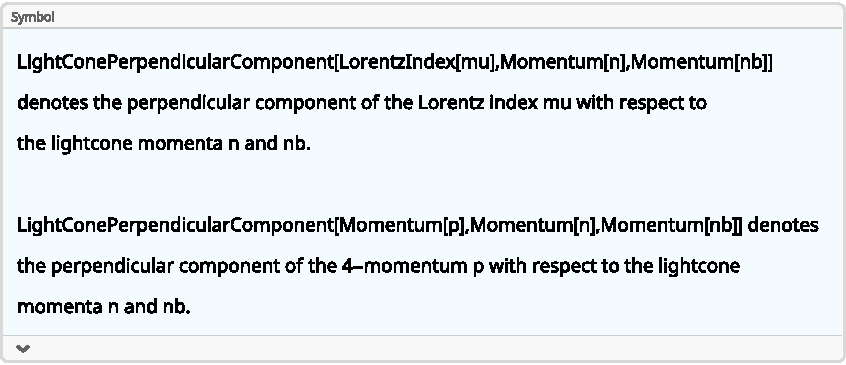
\includegraphics[width=0.6\linewidth]{img/0h6kq1ltbsocf.pdf}
\end{figure}
\FloatBarrier

The pattern introduced for 4-vectors can be also found when working
scalar products, metric tensors or Dirac matrices

\begin{Shaded}
\begin{Highlighting}[]
\OperatorTok{\{}\NormalTok{SPLP}\OperatorTok{[}\FunctionTok{p}\OperatorTok{,} \FunctionTok{q}\OperatorTok{],}\NormalTok{ SPLN}\OperatorTok{[}\FunctionTok{p}\OperatorTok{,} \FunctionTok{q}\OperatorTok{],}\NormalTok{ SPLR}\OperatorTok{[}\FunctionTok{p}\OperatorTok{,} \FunctionTok{q}\OperatorTok{]\}}
\end{Highlighting}
\end{Shaded}

\begin{dmath*}\breakingcomma
\left\{\frac{1}{2} \left(\overline{n}\cdot \overline{p}\right) \left(\overline{\text{nb}}\cdot \overline{q}\right),\frac{1}{2} \left(\overline{n}\cdot \overline{q}\right) \left(\overline{\text{nb}}\cdot \overline{p}\right),\overline{p}\cdot \overline{q}_{\perp }\right\}
\end{dmath*}

\begin{Shaded}
\begin{Highlighting}[]
\OperatorTok{\{}\NormalTok{SPLPD}\OperatorTok{[}\FunctionTok{p}\OperatorTok{,} \FunctionTok{q}\OperatorTok{],}\NormalTok{ SPLND}\OperatorTok{[}\FunctionTok{p}\OperatorTok{,} \FunctionTok{q}\OperatorTok{],}\NormalTok{ SPLRD}\OperatorTok{[}\FunctionTok{p}\OperatorTok{,} \FunctionTok{q}\OperatorTok{]\}}
\end{Highlighting}
\end{Shaded}

\begin{dmath*}\breakingcomma
\left\{\frac{1}{2} (n\cdot p) (\text{nb}\cdot q),\frac{1}{2} (n\cdot q) (\text{nb}\cdot p),p\cdot q_{\perp }\right\}
\end{dmath*}

\begin{Shaded}
\begin{Highlighting}[]
\OperatorTok{\{}\NormalTok{MTLP}\OperatorTok{[}\SpecialCharTok{\textbackslash{}}\OperatorTok{[}\NormalTok{Mu}\OperatorTok{],} \SpecialCharTok{\textbackslash{}}\OperatorTok{[}\NormalTok{Nu}\OperatorTok{]],}\NormalTok{ MTLN}\OperatorTok{[}\SpecialCharTok{\textbackslash{}}\OperatorTok{[}\NormalTok{Mu}\OperatorTok{],} \SpecialCharTok{\textbackslash{}}\OperatorTok{[}\NormalTok{Nu}\OperatorTok{]],}\NormalTok{ MTLR}\OperatorTok{[}\SpecialCharTok{\textbackslash{}}\OperatorTok{[}\NormalTok{Mu}\OperatorTok{],} \SpecialCharTok{\textbackslash{}}\OperatorTok{[}\NormalTok{Nu}\OperatorTok{]]\}}
\end{Highlighting}
\end{Shaded}

\begin{dmath*}\breakingcomma
\left\{\frac{1}{2} \overline{n}^{\nu } \overline{\text{nb}}^{\mu },\frac{1}{2} \overline{n}^{\mu } \overline{\text{nb}}^{\nu },\bar{g}^{\mu \nu }{}_{\perp }\right\}
\end{dmath*}

\begin{Shaded}
\begin{Highlighting}[]
\OperatorTok{\{}\NormalTok{GALP}\OperatorTok{[}\SpecialCharTok{\textbackslash{}}\OperatorTok{[}\NormalTok{Mu}\OperatorTok{]],}\NormalTok{ GALN}\OperatorTok{[}\SpecialCharTok{\textbackslash{}}\OperatorTok{[}\NormalTok{Mu}\OperatorTok{]],}\NormalTok{ GALR}\OperatorTok{[}\SpecialCharTok{\textbackslash{}}\OperatorTok{[}\NormalTok{Mu}\OperatorTok{]]\}}
\end{Highlighting}
\end{Shaded}

\begin{dmath*}\breakingcomma
\left\{\frac{1}{2} \overline{\text{nb}}^{\mu } \bar{\gamma }\cdot \overline{n},\frac{1}{2} \overline{n}^{\mu } \bar{\gamma }\cdot \overline{\text{nb}},\bar{\gamma }^{\mu }{}_{\perp }\right\}
\end{dmath*}

\begin{Shaded}
\begin{Highlighting}[]
\OperatorTok{\{}\NormalTok{GSLP}\OperatorTok{[}\SpecialCharTok{\textbackslash{}}\OperatorTok{[}\NormalTok{Mu}\OperatorTok{]],}\NormalTok{ GSLN}\OperatorTok{[}\SpecialCharTok{\textbackslash{}}\OperatorTok{[}\NormalTok{Mu}\OperatorTok{]],}\NormalTok{ GSLR}\OperatorTok{[}\SpecialCharTok{\textbackslash{}}\OperatorTok{[}\NormalTok{Mu}\OperatorTok{]]\}}
\end{Highlighting}
\end{Shaded}

\begin{dmath*}\breakingcomma
\left\{\frac{1}{2} \bar{\gamma }\cdot \overline{n} \left(\overline{\text{nb}}\cdot \overline{\mu }\right),\frac{1}{2} \left(\overline{n}\cdot \overline{\mu }\right) \bar{\gamma }\cdot \overline{\text{nb}},\bar{\gamma }\cdot \overline{\mu }_{\perp }\right\}
\end{dmath*}

Contracting the full metric tensor with the perpendicular component
returns the latter

\begin{Shaded}
\begin{Highlighting}[]
\NormalTok{MT}\OperatorTok{[}\SpecialCharTok{\textbackslash{}}\OperatorTok{[}\NormalTok{Mu}\OperatorTok{],} \SpecialCharTok{\textbackslash{}}\OperatorTok{[}\NormalTok{Nu}\OperatorTok{]]}\NormalTok{ MTLR}\OperatorTok{[}\SpecialCharTok{\textbackslash{}}\OperatorTok{[}\NormalTok{Mu}\OperatorTok{],} \SpecialCharTok{\textbackslash{}}\OperatorTok{[}\NormalTok{Rho}\OperatorTok{]]}
\SpecialCharTok{\%} \SpecialCharTok{//}\NormalTok{ Contract}
\end{Highlighting}
\end{Shaded}

\begin{dmath*}\breakingcomma
\bar{g}^{\mu \nu } \bar{g}^{\mu \rho }{}_{\perp }
\end{dmath*}

\begin{dmath*}\breakingcomma
\bar{g}^{\nu \rho }{}_{\perp }
\end{dmath*}

The dimensionality of the perpendicular component is \(2\) in
\(4\)-dimensions and \(D-2\) in \(D\)-dimensions

\begin{Shaded}
\begin{Highlighting}[]
\NormalTok{MT}\OperatorTok{[}\SpecialCharTok{\textbackslash{}}\OperatorTok{[}\NormalTok{Mu}\OperatorTok{],} \SpecialCharTok{\textbackslash{}}\OperatorTok{[}\NormalTok{Nu}\OperatorTok{]]}\NormalTok{ MTLR}\OperatorTok{[}\SpecialCharTok{\textbackslash{}}\OperatorTok{[}\NormalTok{Mu}\OperatorTok{],} \SpecialCharTok{\textbackslash{}}\OperatorTok{[}\NormalTok{Nu}\OperatorTok{]]}
\SpecialCharTok{\%} \SpecialCharTok{//}\NormalTok{ Contract}
\end{Highlighting}
\end{Shaded}

\begin{dmath*}\breakingcomma
\bar{g}^{\mu \nu } \bar{g}^{\mu \nu }{}_{\perp }
\end{dmath*}

\begin{dmath*}\breakingcomma
2
\end{dmath*}

\begin{Shaded}
\begin{Highlighting}[]
\NormalTok{MTD}\OperatorTok{[}\SpecialCharTok{\textbackslash{}}\OperatorTok{[}\NormalTok{Mu}\OperatorTok{],} \SpecialCharTok{\textbackslash{}}\OperatorTok{[}\NormalTok{Nu}\OperatorTok{]]}\NormalTok{ MTLRD}\OperatorTok{[}\SpecialCharTok{\textbackslash{}}\OperatorTok{[}\NormalTok{Mu}\OperatorTok{],} \SpecialCharTok{\textbackslash{}}\OperatorTok{[}\NormalTok{Nu}\OperatorTok{]]}
\SpecialCharTok{\%} \SpecialCharTok{//}\NormalTok{ Contract}
\end{Highlighting}
\end{Shaded}

\begin{dmath*}\breakingcomma
g^{\mu \nu } g^{\mu \nu }{}_{\perp }
\end{dmath*}

\begin{dmath*}\breakingcomma
D-2
\end{dmath*}

\subsection{Dirac matrices with light-cone
components}\label{dirac-matrices-with-light-cone-components}

Dirac algebra involving matrices contracted to light-cone momenta or
having particular light-cone components is fully supported. The general
strategy followed by \texttt{DiracSimplify} is to move all perpendicular
components to the very right of the chain.

\begin{Shaded}
\begin{Highlighting}[]
\NormalTok{ex1 }\ExtensionTok{=}\NormalTok{ GALR}\OperatorTok{[}\FunctionTok{p}\OperatorTok{]}\NormalTok{ . GA}\OperatorTok{[}\SpecialCharTok{\textbackslash{}}\OperatorTok{[}\NormalTok{Mu}\OperatorTok{],} \SpecialCharTok{\textbackslash{}}\OperatorTok{[}\NormalTok{Nu}\OperatorTok{]]}
\end{Highlighting}
\end{Shaded}

\begin{dmath*}\breakingcomma
\bar{\gamma }^p{}_{\perp }.\bar{\gamma }^{\mu }.\bar{\gamma }^{\nu }
\end{dmath*}

\begin{Shaded}
\begin{Highlighting}[]
\NormalTok{ex1 }\SpecialCharTok{//}\NormalTok{ DiracSimplify}
\end{Highlighting}
\end{Shaded}

\begin{dmath*}\breakingcomma
-\frac{1}{2} \overline{n}^{\mu } \left(\bar{\gamma }\cdot \overline{\text{nb}}\right).\bar{\gamma }^p{}_{\perp }.\bar{\gamma }^{\nu }{}_{\perp }-\frac{1}{2} \overline{\text{nb}}^{\mu } \left(\bar{\gamma }\cdot \overline{n}\right).\bar{\gamma }^p{}_{\perp }.\bar{\gamma }^{\nu }{}_{\perp }+\frac{1}{2} \overline{n}^{\nu } \left(\bar{\gamma }\cdot \overline{\text{nb}}\right).\bar{\gamma }^p{}_{\perp }.\bar{\gamma }^{\mu }{}_{\perp }+\frac{1}{4} \overline{n}^{\nu } \overline{\text{nb}}^{\mu } \left(\bar{\gamma }\cdot \overline{n}\right).\left(\bar{\gamma }\cdot \overline{\text{nb}}\right).\bar{\gamma }^p{}_{\perp }+\frac{1}{2} \overline{\text{nb}}^{\nu } \left(\bar{\gamma }\cdot \overline{n}\right).\bar{\gamma }^p{}_{\perp }.\bar{\gamma }^{\mu }{}_{\perp }-\frac{1}{4} \overline{n}^{\mu } \overline{\text{nb}}^{\nu } \left(\bar{\gamma }\cdot \overline{n}\right).\left(\bar{\gamma }\cdot \overline{\text{nb}}\right).\bar{\gamma }^p{}_{\perp }+\overline{n}^{\mu } \overline{\text{nb}}^{\nu } \bar{\gamma }^p{}_{\perp }+\bar{\gamma }^p{}_{\perp }.\bar{\gamma }^{\mu }{}_{\perp }.\bar{\gamma }^{\nu }{}_{\perp }
\end{dmath*}

\begin{Shaded}
\begin{Highlighting}[]
\NormalTok{ex2 }\ExtensionTok{=}\NormalTok{ GALR}\OperatorTok{[}\FunctionTok{p}\OperatorTok{]}\NormalTok{ . GA}\OperatorTok{[}\SpecialCharTok{\textbackslash{}}\OperatorTok{[}\NormalTok{Mu}\OperatorTok{],} \SpecialCharTok{\textbackslash{}}\OperatorTok{[}\NormalTok{Nu}\OperatorTok{]]}\NormalTok{ . GALR}\OperatorTok{[}\FunctionTok{p}\OperatorTok{]}
\end{Highlighting}
\end{Shaded}

\begin{dmath*}\breakingcomma
\bar{\gamma }^p{}_{\perp }.\bar{\gamma }^{\mu }.\bar{\gamma }^{\nu }.\bar{\gamma }^p{}_{\perp }
\end{dmath*}

\begin{Shaded}
\begin{Highlighting}[]
\NormalTok{ex2 }\SpecialCharTok{//}\NormalTok{ DiracSimplify}
\end{Highlighting}
\end{Shaded}

\begin{dmath*}\breakingcomma
-2 \bar{\gamma }^{\mu }{}_{\perp }.\bar{\gamma }^{\nu }{}_{\perp }+4 \bar{g}^{\mu \nu }{}_{\perp }+\frac{1}{2} \overline{n}^{\nu } \overline{\text{nb}}^{\mu } \left(\bar{\gamma }\cdot \overline{n}\right).\left(\bar{\gamma }\cdot \overline{\text{nb}}\right)-\frac{1}{2} \overline{n}^{\mu } \overline{\text{nb}}^{\nu } \left(\bar{\gamma }\cdot \overline{n}\right).\left(\bar{\gamma }\cdot \overline{\text{nb}}\right)+2 \overline{n}^{\mu } \overline{\text{nb}}^{\nu }
\end{dmath*}

Notice that when entering particular light-cone components of Dirac
matrices, the standard trick for entering multiple indices does not
work. This is because the 2nd and 3rd arguments are reserved for
user-specified light-cone vectors

\begin{Shaded}
\begin{Highlighting}[]
\NormalTok{GALR}\OperatorTok{[}\NormalTok{mu1}\OperatorTok{,}\NormalTok{ myN}\OperatorTok{,}\NormalTok{ myNB}\OperatorTok{]}
\SpecialCharTok{\%} \SpecialCharTok{//}\NormalTok{ FCI }\SpecialCharTok{//} \FunctionTok{StandardForm}
\end{Highlighting}
\end{Shaded}

\begin{dmath*}\breakingcomma
\bar{\gamma }^{\text{mu1}}{}_{\perp }
\end{dmath*}

\begin{Shaded}
\begin{Highlighting}[]
\CommentTok{(*DiracGamma[LightConePerpendicularComponent[LorentzIndex[mu1], Momentum[myN], Momentum[myNB]]]*)}
\end{Highlighting}
\end{Shaded}

Instead, you should put your list of indices into curly brackets

\begin{Shaded}
\begin{Highlighting}[]
\NormalTok{GALR}\OperatorTok{[\{}\SpecialCharTok{\textbackslash{}}\OperatorTok{[}\NormalTok{Mu}\OperatorTok{],} \SpecialCharTok{\textbackslash{}}\OperatorTok{[}\NormalTok{Nu}\OperatorTok{],} \SpecialCharTok{\textbackslash{}}\OperatorTok{[}\NormalTok{Rho}\OperatorTok{]\}]}
\end{Highlighting}
\end{Shaded}

\begin{dmath*}\breakingcomma
\bar{\gamma }^{\mu }{}_{\perp }.\bar{\gamma }^{\nu }{}_{\perp }.\bar{\gamma }^{\rho }{}_{\perp }
\end{dmath*}

\begin{Shaded}
\begin{Highlighting}[]
\NormalTok{ex3 }\ExtensionTok{=}\NormalTok{ GALR}\OperatorTok{[}\FunctionTok{p}\OperatorTok{]}\NormalTok{ . GALR}\OperatorTok{[\{}\SpecialCharTok{\textbackslash{}}\OperatorTok{[}\NormalTok{Mu}\OperatorTok{],} \SpecialCharTok{\textbackslash{}}\OperatorTok{[}\NormalTok{Nu}\OperatorTok{]\}]}\NormalTok{ . GALR}\OperatorTok{[}\FunctionTok{p}\OperatorTok{]}
\end{Highlighting}
\end{Shaded}

\begin{dmath*}\breakingcomma
\bar{\gamma }^p{}_{\perp }.\bar{\gamma }^{\mu }{}_{\perp }.\bar{\gamma }^{\nu }{}_{\perp }.\bar{\gamma }^p{}_{\perp }
\end{dmath*}

\begin{Shaded}
\begin{Highlighting}[]
\NormalTok{ex3 }\SpecialCharTok{//}\NormalTok{ DiracSimplify}
\end{Highlighting}
\end{Shaded}

\begin{dmath*}\breakingcomma
4 \bar{g}^{\mu \nu }{}_{\perp }-2 \bar{\gamma }^{\mu }{}_{\perp }.\bar{\gamma }^{\nu }{}_{\perp }
\end{dmath*}

\begin{Shaded}
\begin{Highlighting}[]
\NormalTok{ex4 }\ExtensionTok{=}\NormalTok{ DiracTrace}\OperatorTok{[}\NormalTok{GA}\OperatorTok{[}\SpecialCharTok{\textbackslash{}}\OperatorTok{[}\NormalTok{Rho}\OperatorTok{],} \SpecialCharTok{\textbackslash{}}\OperatorTok{[}\NormalTok{Sigma}\OperatorTok{]]}\NormalTok{ . GALR}\OperatorTok{[\{}\SpecialCharTok{\textbackslash{}}\OperatorTok{[}\NormalTok{Mu}\OperatorTok{],} \SpecialCharTok{\textbackslash{}}\OperatorTok{[}\NormalTok{Nu}\OperatorTok{]\}]]}
\end{Highlighting}
\end{Shaded}

\begin{dmath*}\breakingcomma
\text{tr}\left(\bar{\gamma }^{\rho }.\bar{\gamma }^{\sigma }.\bar{\gamma }^{\mu }{}_{\perp }.\bar{\gamma }^{\nu }{}_{\perp }\right)
\end{dmath*}

\begin{Shaded}
\begin{Highlighting}[]
\NormalTok{ex4 }\SpecialCharTok{//}\NormalTok{ DiracSimplify}
\end{Highlighting}
\end{Shaded}

\begin{dmath*}\breakingcomma
4 \bar{g}^{\mu \sigma }{}_{\perp } \bar{g}^{\nu \rho }{}_{\perp }-4 \bar{g}^{\mu \rho }{}_{\perp } \bar{g}^{\nu \sigma }{}_{\perp }+4 \bar{g}^{\rho \sigma } \bar{g}^{\mu \nu }{}_{\perp }
\end{dmath*}

\begin{Shaded}
\begin{Highlighting}[]
\NormalTok{ex5 }\ExtensionTok{=}\NormalTok{ DiracTrace}\OperatorTok{[}\NormalTok{GA}\OperatorTok{[}\SpecialCharTok{\textbackslash{}}\OperatorTok{[}\NormalTok{Rho}\OperatorTok{],} \SpecialCharTok{\textbackslash{}}\OperatorTok{[}\NormalTok{Sigma}\OperatorTok{]]}\NormalTok{ . GA}\OperatorTok{[}\DecValTok{5}\OperatorTok{]}\NormalTok{ . GALR}\OperatorTok{[\{}\SpecialCharTok{\textbackslash{}}\OperatorTok{[}\NormalTok{Mu}\OperatorTok{],} \SpecialCharTok{\textbackslash{}}\OperatorTok{[}\NormalTok{Nu}\OperatorTok{]\}]]}
\end{Highlighting}
\end{Shaded}

\begin{dmath*}\breakingcomma
\text{tr}\left(\bar{\gamma }^{\rho }.\bar{\gamma }^{\sigma }.\bar{\gamma }^5.\bar{\gamma }^{\mu }{}_{\perp }.\bar{\gamma }^{\nu }{}_{\perp }\right)
\end{dmath*}

\begin{Shaded}
\begin{Highlighting}[]
\NormalTok{ex5 }\SpecialCharTok{//}\NormalTok{ DiracSimplify}
\end{Highlighting}
\end{Shaded}

\begin{dmath*}\breakingcomma
2 i \overline{n}^{\rho } \bar{\epsilon }^{\mu _{\perp }\nu _{\perp }\sigma _{\perp }\;\overline{\text{nb}}}+2 i \overline{\text{nb}}^{\rho } \bar{\epsilon }^{\mu _{\perp }\nu _{\perp }\sigma _{\perp }\overline{n}}-2 i \overline{n}^{\sigma } \bar{\epsilon }^{\mu _{\perp }\nu _{\perp }\rho _{\perp }\;\overline{\text{nb}}}-i \overline{n}^{\sigma } \overline{\text{nb}}^{\rho } \bar{\epsilon }^{\mu _{\perp }\nu _{\perp }\overline{n}\;\overline{\text{nb}}}-2 i \overline{\text{nb}}^{\sigma } \bar{\epsilon }^{\mu _{\perp }\nu _{\perp }\rho _{\perp }\overline{n}}+i \overline{n}^{\rho } \overline{\text{nb}}^{\sigma } \bar{\epsilon }^{\mu _{\perp }\nu _{\perp }\overline{n}\;\overline{\text{nb}}}-4 i \bar{\epsilon }^{\mu _{\perp }\nu _{\perp }\rho _{\perp }\sigma _{\perp }}
\end{dmath*}

In order to handle Dirac matrices involving light-cone components
effectively, one needs to define some ordering. The current (hard-coded)
choice is that the perpendicular component always get anticommuted to
the very right of each Dirac chain, while every remaining occurence of
\((\gamma \cdot \bar{n}) (\gamma \cdot n)\) is changed to
\((\gamma \cdot n) (\gamma \cdot \bar{n})\).

\subsection{Introducing light-cone components by
hand}\label{introducing-light-cone-components-by-hand}

In some calculations one might end up with a mixture of explicit
light-cone components and generic Lorentz tensors. If those tensors
admit a particularly simple representation in terms of light-cone
components, it can be enforced using the function
\texttt{ToLightConeComponents}

For example, the following expression cannot be simplified any further

\begin{Shaded}
\begin{Highlighting}[]
\NormalTok{ex6 }\ExtensionTok{=}\NormalTok{ GS}\OperatorTok{[}\NormalTok{nb}\OperatorTok{,}\NormalTok{ vp}\OperatorTok{]}
\end{Highlighting}
\end{Shaded}

\begin{dmath*}\breakingcomma
\left(\bar{\gamma }\cdot \overline{\text{nb}}\right).\left(\bar{\gamma }\cdot \overline{\text{vp}}\right)
\end{dmath*}

Now let us suppose that \((v')^{\mu}\) can be actually written as
\(\alpha n^\mu + \bar{n}^{\mu}/(4 \alpha)\). We can implement this as
follows

\begin{Shaded}
\begin{Highlighting}[]
\NormalTok{SP}\OperatorTok{[}\NormalTok{vp}\OperatorTok{,}\NormalTok{ nb}\OperatorTok{]} \ExtensionTok{=} \DecValTok{2}\SpecialCharTok{*}\NormalTok{alpha;}
\NormalTok{SP}\OperatorTok{[}\NormalTok{vp}\OperatorTok{,} \FunctionTok{n}\OperatorTok{]} \ExtensionTok{=} \DecValTok{2}\SpecialCharTok{*}\DecValTok{1}\SpecialCharTok{/}\NormalTok{(}\DecValTok{4}\NormalTok{ alpha);}
\NormalTok{LightConePerpendicularComponent}\OperatorTok{[}\NormalTok{Momentum}\OperatorTok{[}\NormalTok{vp}\OperatorTok{],}\NormalTok{ Momentum}\OperatorTok{[}\FunctionTok{n}\OperatorTok{],}\NormalTok{ Momentum}\OperatorTok{[}\NormalTok{nb}\OperatorTok{]]} \ExtensionTok{=} \DecValTok{0}\NormalTok{;}
\end{Highlighting}
\end{Shaded}

\begin{Shaded}
\begin{Highlighting}[]
\NormalTok{FV}\OperatorTok{[}\NormalTok{vp}\OperatorTok{,}\NormalTok{ mu}\OperatorTok{]}
\SpecialCharTok{\%} \SpecialCharTok{//}\NormalTok{ ToLightConeComponents}
\end{Highlighting}
\end{Shaded}

\begin{dmath*}\breakingcomma
\overline{\text{vp}}^{\text{mu}}
\end{dmath*}

\begin{dmath*}\breakingcomma
\text{alpha} \overline{n}^{\text{mu}}+\frac{\overline{\text{nb}}^{\text{mu}}}{4 \;\text{alpha}}
\end{dmath*}

However, this will not make FeynCalc automatically simplify the Dirac
chain

\begin{Shaded}
\begin{Highlighting}[]
\NormalTok{ex6 }\SpecialCharTok{//}\NormalTok{ DiracSimplify}
\end{Highlighting}
\end{Shaded}

\begin{dmath*}\breakingcomma
\left(\bar{\gamma }\cdot \overline{\text{nb}}\right).\left(\bar{\gamma }\cdot \overline{\text{vp}}\right)
\end{dmath*}

Using \texttt{ToLightConeComponents} we can explicitly rewrite
\texttt{vp} in the chain in terms of the light-cone components and hence
enforce the desired simplification. In fact, the function will also
automatically simplify some common expressions such
\(\gamma \cdot \bar{n} \gamma \cdot \bar{n} = \gamma \cdot n \gamma \cdot n = 0\)

\begin{Shaded}
\begin{Highlighting}[]
\NormalTok{ex6 }\SpecialCharTok{//}\NormalTok{ ToLightConeComponents}
\SpecialCharTok{\%} \SpecialCharTok{//}\NormalTok{ DiracSimplify}
\end{Highlighting}
\end{Shaded}

\begin{dmath*}\breakingcomma
\text{alpha} \left(\bar{\gamma }\cdot \overline{\text{nb}}\right).\left(\bar{\gamma }\cdot \overline{n}\right)
\end{dmath*}

\begin{dmath*}\breakingcomma
4 \;\text{alpha}-\text{alpha} \left(\bar{\gamma }\cdot \overline{n}\right).\left(\bar{\gamma }\cdot \overline{\text{nb}}\right)
\end{dmath*}

Such simplifications inside \texttt{ToLightConeComponents} can be
disabled using the option \texttt{DotSimplify}

\begin{Shaded}
\begin{Highlighting}[]
\NormalTok{ex6 }\SpecialCharTok{//}\NormalTok{ ToLightConeComponents}\OperatorTok{[}\NormalTok{\#}\OperatorTok{,}\NormalTok{ DotSimplify }\OtherTok{{-}\textgreater{}} \ConstantTok{False}\OperatorTok{]}\NormalTok{ \&}
\SpecialCharTok{\%} \SpecialCharTok{//}\NormalTok{ DiracSimplify}
\end{Highlighting}
\end{Shaded}

\begin{dmath*}\breakingcomma
\left(\bar{\gamma }\cdot \overline{\text{nb}}\right).\left(\text{alpha} \bar{\gamma }\cdot \overline{n}+\frac{\bar{\gamma }\cdot \overline{\text{nb}}}{4 \;\text{alpha}}\right)
\end{dmath*}

\begin{dmath*}\breakingcomma
4 \;\text{alpha}-\text{alpha} \left(\bar{\gamma }\cdot \overline{n}\right).\left(\bar{\gamma }\cdot \overline{\text{nb}}\right)
\end{dmath*}

\subsection{Reductions of loop integrals with numerators involving
light-cone
components}\label{reductions-of-loop-integrals-with-numerators-involving-light-cone-components}

\begin{Shaded}
\begin{Highlighting}[]
\NormalTok{int }\ExtensionTok{=}\NormalTok{ FVLRD}\OperatorTok{[}\FunctionTok{p}\OperatorTok{,} \SpecialCharTok{\textbackslash{}}\OperatorTok{[}\NormalTok{Mu}\OperatorTok{]]}\NormalTok{ SFAD}\OperatorTok{[}\FunctionTok{p}\OperatorTok{,} \FunctionTok{p} \SpecialCharTok{{-}} \FunctionTok{q}\OperatorTok{]}
\end{Highlighting}
\end{Shaded}

\begin{dmath*}\breakingcomma
\frac{p^{\mu }{}_{\perp }}{(p^2+i \eta ).((p-q)^2+i \eta )}
\end{dmath*}

\begin{Shaded}
\begin{Highlighting}[]
\NormalTok{TID}\OperatorTok{[}\NormalTok{int}\OperatorTok{,} \FunctionTok{p}\OperatorTok{]}
\end{Highlighting}
\end{Shaded}

\begin{dmath*}\breakingcomma
\frac{q^{\mu }{}_{\perp }}{2 (p^2+i \eta ).((p-q)^2+i \eta )}
\end{dmath*}

\subsection{Differentiations}\label{differentiations}

\texttt{FourDivergence} cannot yet differentiate w.r.t light-cone
components directly. However, the same effect can be easily achieved by
first differentiating w.r.t the usual 4-momentum and then contracting
the free index with the corresponding metric tensor

\begin{Shaded}
\begin{Highlighting}[]
\NormalTok{ex }\ExtensionTok{=}\NormalTok{ FV}\OperatorTok{[}\NormalTok{p1}\OperatorTok{,} \SpecialCharTok{\textbackslash{}}\OperatorTok{[}\NormalTok{Mu}\OperatorTok{]]}\SpecialCharTok{/}\NormalTok{SP}\OperatorTok{[}\NormalTok{p1}\OperatorTok{]}
\end{Highlighting}
\end{Shaded}

\begin{dmath*}\breakingcomma
\frac{\overline{\text{p1}}^{\mu }}{\overline{\text{p1}}^2}
\end{dmath*}

Differentiating w.r.t \(p_{1,+}\), \(p_{1,-}\) or \(p_{1,\perp}\)

\begin{Shaded}
\begin{Highlighting}[]
\NormalTok{MTLN}\OperatorTok{[}\SpecialCharTok{\textbackslash{}}\OperatorTok{[}\NormalTok{Nu}\OperatorTok{],} \SpecialCharTok{\textbackslash{}}\OperatorTok{[}\NormalTok{Rho}\OperatorTok{]]}\NormalTok{ FourDivergence}\OperatorTok{[}\NormalTok{ex}\OperatorTok{,}\NormalTok{ FV}\OperatorTok{[}\NormalTok{p1}\OperatorTok{,} \SpecialCharTok{\textbackslash{}}\OperatorTok{[}\NormalTok{Rho}\OperatorTok{]]]} \SpecialCharTok{//}\NormalTok{ Contract}
\end{Highlighting}
\end{Shaded}

\begin{dmath*}\breakingcomma
\frac{\overline{n}^{\nu } \overline{\text{nb}}^{\mu }}{2 \overline{\text{p1}}^2}-\frac{\overline{n}^{\nu } \overline{\text{p1}}^{\mu } \left(\overline{\text{nb}}\cdot \overline{\text{p1}}\right)}{\overline{\text{p1}}^4}
\end{dmath*}

\begin{Shaded}
\begin{Highlighting}[]
\NormalTok{MTLP}\OperatorTok{[}\SpecialCharTok{\textbackslash{}}\OperatorTok{[}\NormalTok{Nu}\OperatorTok{],} \SpecialCharTok{\textbackslash{}}\OperatorTok{[}\NormalTok{Rho}\OperatorTok{]]}\NormalTok{ FourDivergence}\OperatorTok{[}\NormalTok{ex}\OperatorTok{,}\NormalTok{ FV}\OperatorTok{[}\NormalTok{p1}\OperatorTok{,} \SpecialCharTok{\textbackslash{}}\OperatorTok{[}\NormalTok{Rho}\OperatorTok{]]]} \SpecialCharTok{//}\NormalTok{ Contract}
\end{Highlighting}
\end{Shaded}

\begin{dmath*}\breakingcomma
\frac{\overline{n}^{\mu } \overline{\text{nb}}^{\nu }}{2 \overline{\text{p1}}^2}-\frac{\overline{\text{nb}}^{\nu } \overline{\text{p1}}^{\mu } \left(\overline{n}\cdot \overline{\text{p1}}\right)}{\overline{\text{p1}}^4}
\end{dmath*}

\begin{Shaded}
\begin{Highlighting}[]
\NormalTok{MTLR}\OperatorTok{[}\SpecialCharTok{\textbackslash{}}\OperatorTok{[}\NormalTok{Nu}\OperatorTok{],} \SpecialCharTok{\textbackslash{}}\OperatorTok{[}\NormalTok{Rho}\OperatorTok{]]}\NormalTok{ FourDivergence}\OperatorTok{[}\NormalTok{ex}\OperatorTok{,}\NormalTok{ FV}\OperatorTok{[}\NormalTok{p1}\OperatorTok{,} \SpecialCharTok{\textbackslash{}}\OperatorTok{[}\NormalTok{Rho}\OperatorTok{]]]} \SpecialCharTok{//}\NormalTok{ Contract}
\end{Highlighting}
\end{Shaded}

\begin{dmath*}\breakingcomma
\frac{\bar{g}^{\mu \nu }{}_{\perp }}{\overline{\text{p1}}^2}-\frac{2 \overline{\text{p1}}^{\mu } \overline{\text{p1}}^{\nu }{}_{\perp }}{\overline{\text{p1}}^4}
\end{dmath*}
\end{document}
